\chapter{Implementacija i korisničko sučelje}
		
		
		\section{Korištene tehnologije i alati}
		
			Kao dogovoren način razmjenjivanja ideja i dogovaranja oko projekta odabrana je 
			aplikacija Whatsapp \textbf{https://www.whatsapp.com/}. Github \textbf{https://github.com/}
			je odabran kao sustav za upravljanje cjelokupnim kodom projekta, a za izradu 
			svih dijagrama (sekvencijskih dijagrama, dijagrama razreda, dijagrama komponenti i sl.) 
			korišten je alat Visual Paradigm \textbf{https://online.visual-paradigm.com/}.
			
			Za razvojnu okolinu odabran je Visual Studio Code \textbf{https://code.visualstudio.com/}
			iz razloga što je jednostavan za korištenje jer pruža mogućnost pametnog dovršavanja
			na temelju vrsta varijabli i definicija funkcija za koju je zaslužan IntelliSense.
			Uz to sve, VSC je prilagodljiva okolina s puno ekstenzija, a i lako se povezuje 
			s GitHubom.
			
			Aplikacija je razvijena pomoću Java Spring Boot \textbf{https://spring.io/projects/spring-boot/},
			a korišten programski jezik je Java \textbf{https://www.java.com/en/}, verzija 17. 
			Za frontend je korišten programski jezik JavaScript \textbf{https://www.javascript.com/}, preciznije, 
			jezik TypeScript \textbf{https://www.typescriptlang.org/} koji je nadogradnja već
			postojećeg JavaScripta te biblioteka React \textbf{https://react.dev/}.
			Korištenjem TypeScripta omogućeno je dodavanje tipova i dodatnih mogućnosti nego samo
			koristeći JavaScript. Upotrebljena je i biblioteka ReactQuery koja omogućuje
			automatsko ažuriranje podataka - implementira logiku za osvježavanje i predmemoriranje 
			podataka, kao i za njihovu invalidaciju. Uz sve navedeno, korištene su i
			biblioteke UI komponenti ChakraUI i TailwindCSS za stiliziranje i dizajn korisničkog sučelja.
			
			Za bazu podataka korišten je Postgres \textbf{https://www.postgresql.org/} koja se 
			pokreće pomoću Dockera \textbf{https://www.docker.com/}, odnosno Docker containera.
			
			
			\eject 
		
	
		\section{Ispitivanje programskog rješenja}
			
			
			\subsection{Ispitivanje komponenti}
			\textit{Potrebno je provesti ispitivanje jedinica (engl. unit testing) nad razredima koji implementiraju temeljne funkcionalnosti. Razraditi \textbf{minimalno 6 ispitnih slučajeva} u kojima će se ispitati redovni slučajevi, rubni uvjeti te izazivanje pogreške (engl. exception throwing). Poželjno je stvoriti i ispitni slučaj koji koristi funkcionalnosti koje nisu implementirane. Potrebno je priložiti izvorni kôd svih ispitnih slučajeva te prikaz rezultata izvođenja ispita u razvojnom okruženju (prolaz/pad ispita). }
			
			
			
			\subsection{Ispitivanje sustava}
			
			Ispitivanje sustava izvedeno je u programskom jeziku Python koristeći Selenium WebDriver. Priloženi kodovi su u nastavku, ali prije toga je izdvojen zajednički kod koji koriste svi testovi.
			
			\begin{figure}[H]
				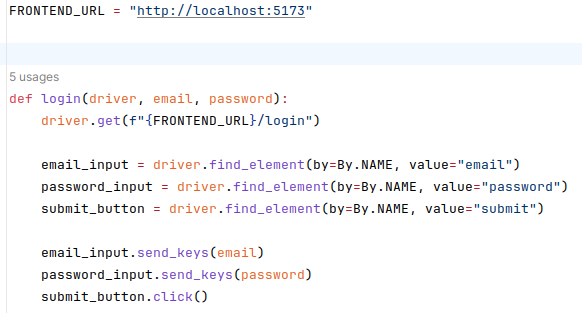
\includegraphics[width=\textwidth]{slike/selenium_common.png}
				\centering
				\caption{Zajednički kod testova}
				\label{fig:zajednicki-kod-testova}
			\end{figure}
			
			Prvi test ispituje pokušaj prijave s krivim podatcima. Očekivani je da se putanja ne promijeni te da se pojavi obavijest u obliku \textit{Toast}-a koja daje više informacija o greški.   
			
			\begin{figure}[H]
				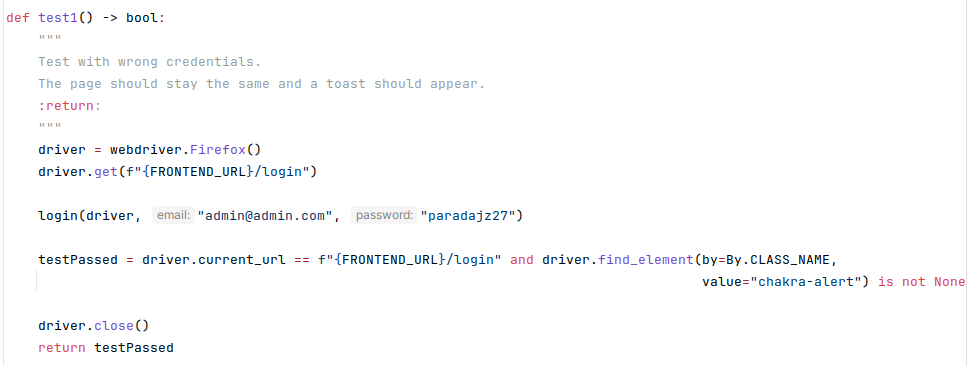
\includegraphics[width=\textwidth]{slike/selenium_test1.png}
				\centering
				\caption{Izvorni kod 1. testa}
				\label{fig:izvorni-kod-testa-1}
			\end{figure}
		
			Drugi test ispituje pokušaj prijave s ispravnim podatcima. Očekivano ponašanje je da se putanja promijeni te da gumb "Logout" bude vidljiv.
			
			\begin{figure}[H]
				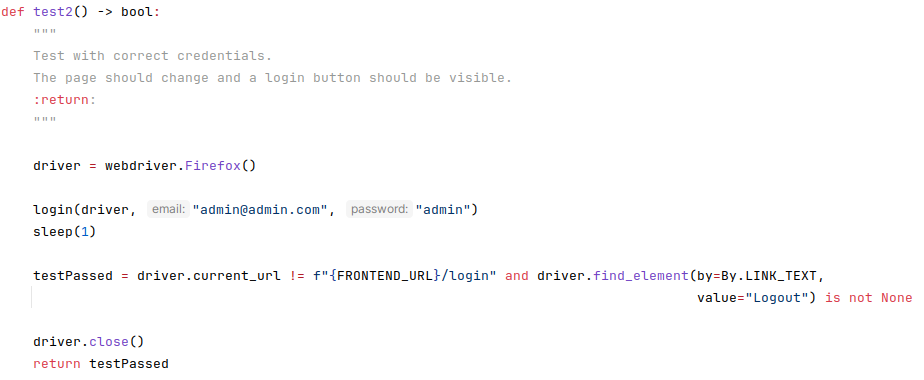
\includegraphics[width=\textwidth]{slike/selenium_test2.png}
				\centering
				\caption{Izvorni kod 2. testa}
				\label{fig:izvorni-kod-testa-2}
			\end{figure}
		
			Treći test ispituje stvaranje transportne kompanije. Očekivano ponašanje je povećanje broja redaka u tablici koja prikazuje transportne kompanije za 1.
		
			\begin{figure}[H]
				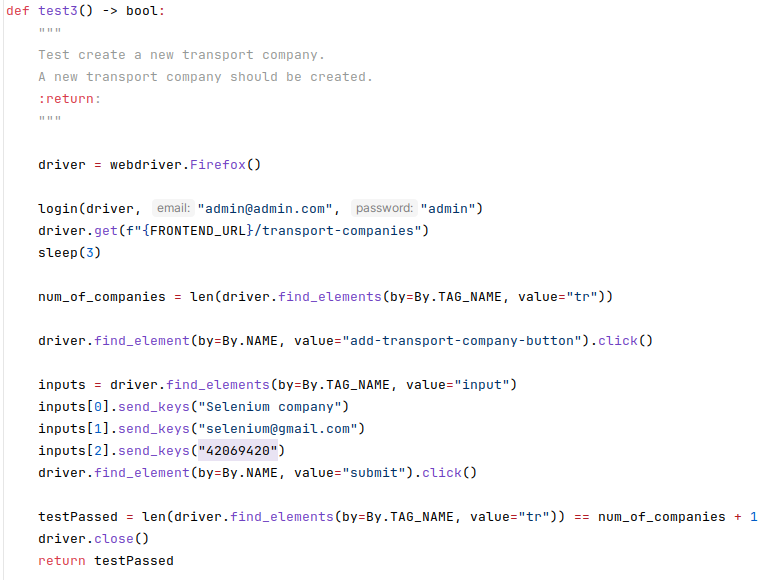
\includegraphics[width=\textwidth]{slike/selenium_test3.png}
				\centering
				\caption{Izvorni kod 3. testa}
				\label{fig:izvorni-kod-testa-3}
			\end{figure}
		
			Četvrti test ispituje brisanje transportne kompanije. Očekivano ponašanje je smanjenje broja redaka u tablici koja prikazuje transportne kompanije za 1
		
			\begin{figure}[H]
				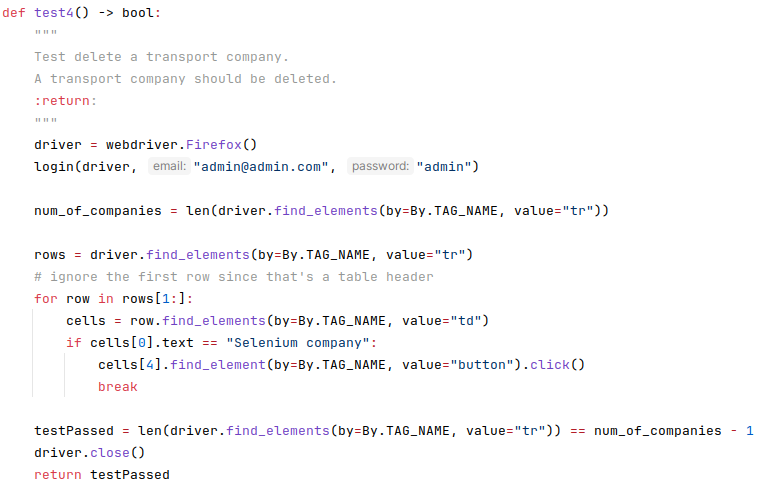
\includegraphics[width=\textwidth]{slike/selenium_test4.png}
				\centering
				\caption{Izvorni kod 4. testa}
				\label{fig:izvorni-kod-testa-4}
			\end{figure}
		
			Peti test ispituje odjavljivanje korisnika. Očekivano ponašanje je promjena putanje na "/login".
			
			\begin{figure}[H]
				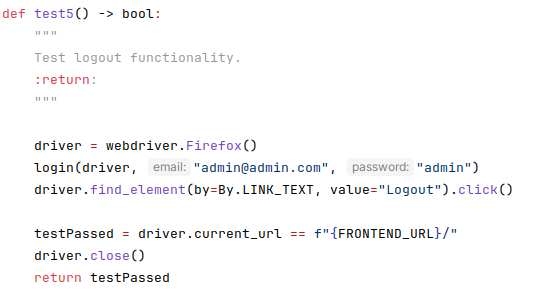
\includegraphics[width=\textwidth]{slike/selenium_test5.png}
				\centering
				\caption{Izvorni kod 5. testa}
				\label{fig:izvorni-kod-testa-5}
			\end{figure}
		
			Kod koji prikazuje kako su testovi pokrenuti.
			
			\begin{figure}[H]
				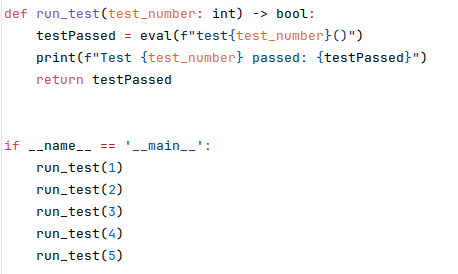
\includegraphics[width=\textwidth]{slike/selenium_running.png}
				\centering
				\caption{Izvršavanje testova}
				\label{fig:izvrsavanje-testova}
			\end{figure}
		
			Rezultati izvršenih testova.
			
			\begin{figure}[H]
				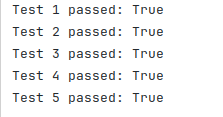
\includegraphics[width=\textwidth]{slike/selenium_results.png}
				\centering
				\caption{Rezultati testova}
				\label{fig:rezultati-testova}
			\end{figure}
				
			
			
			
			\eject 
		
		
		\section{Dijagram razmještaja}
			
			
			Dijagram razmještaja na slici \ref{fig:implementacija_dijagram_razmjestaja} prikazuje topologiju sklopovlja i programsku potporu web-aplikacije. Sustav je baziran na arhitekturi "klijent-poslužitelj". Komunikacija između računala korisnika i frontend poslužiteljskog računala, kao i između frontend i backend poslužiteljskog računala, odvija se preko HTTP veze. Korisnici pristupaju web-aplikaciji koristeći web preglednik te im frontend poslužiteljsko računalo, na kojemu se nalazi frontend web poslužitelj, daje odgovarajući prikaz. Na backend poslužiteljskom računalu se nalazi backend web poslužitelj te Spring aplikacija, a Postgres baza nalazi se na poslužiteljskom računalu baze podataka koje je povezano s backend poslužiteljskim računalom. Backend poslužiteljsko računalo također je spojeno na poslužiteljsko računalo vanjskog servisa, koje je postavljeno na sličan način.
			
			\begin{figure}[H]
				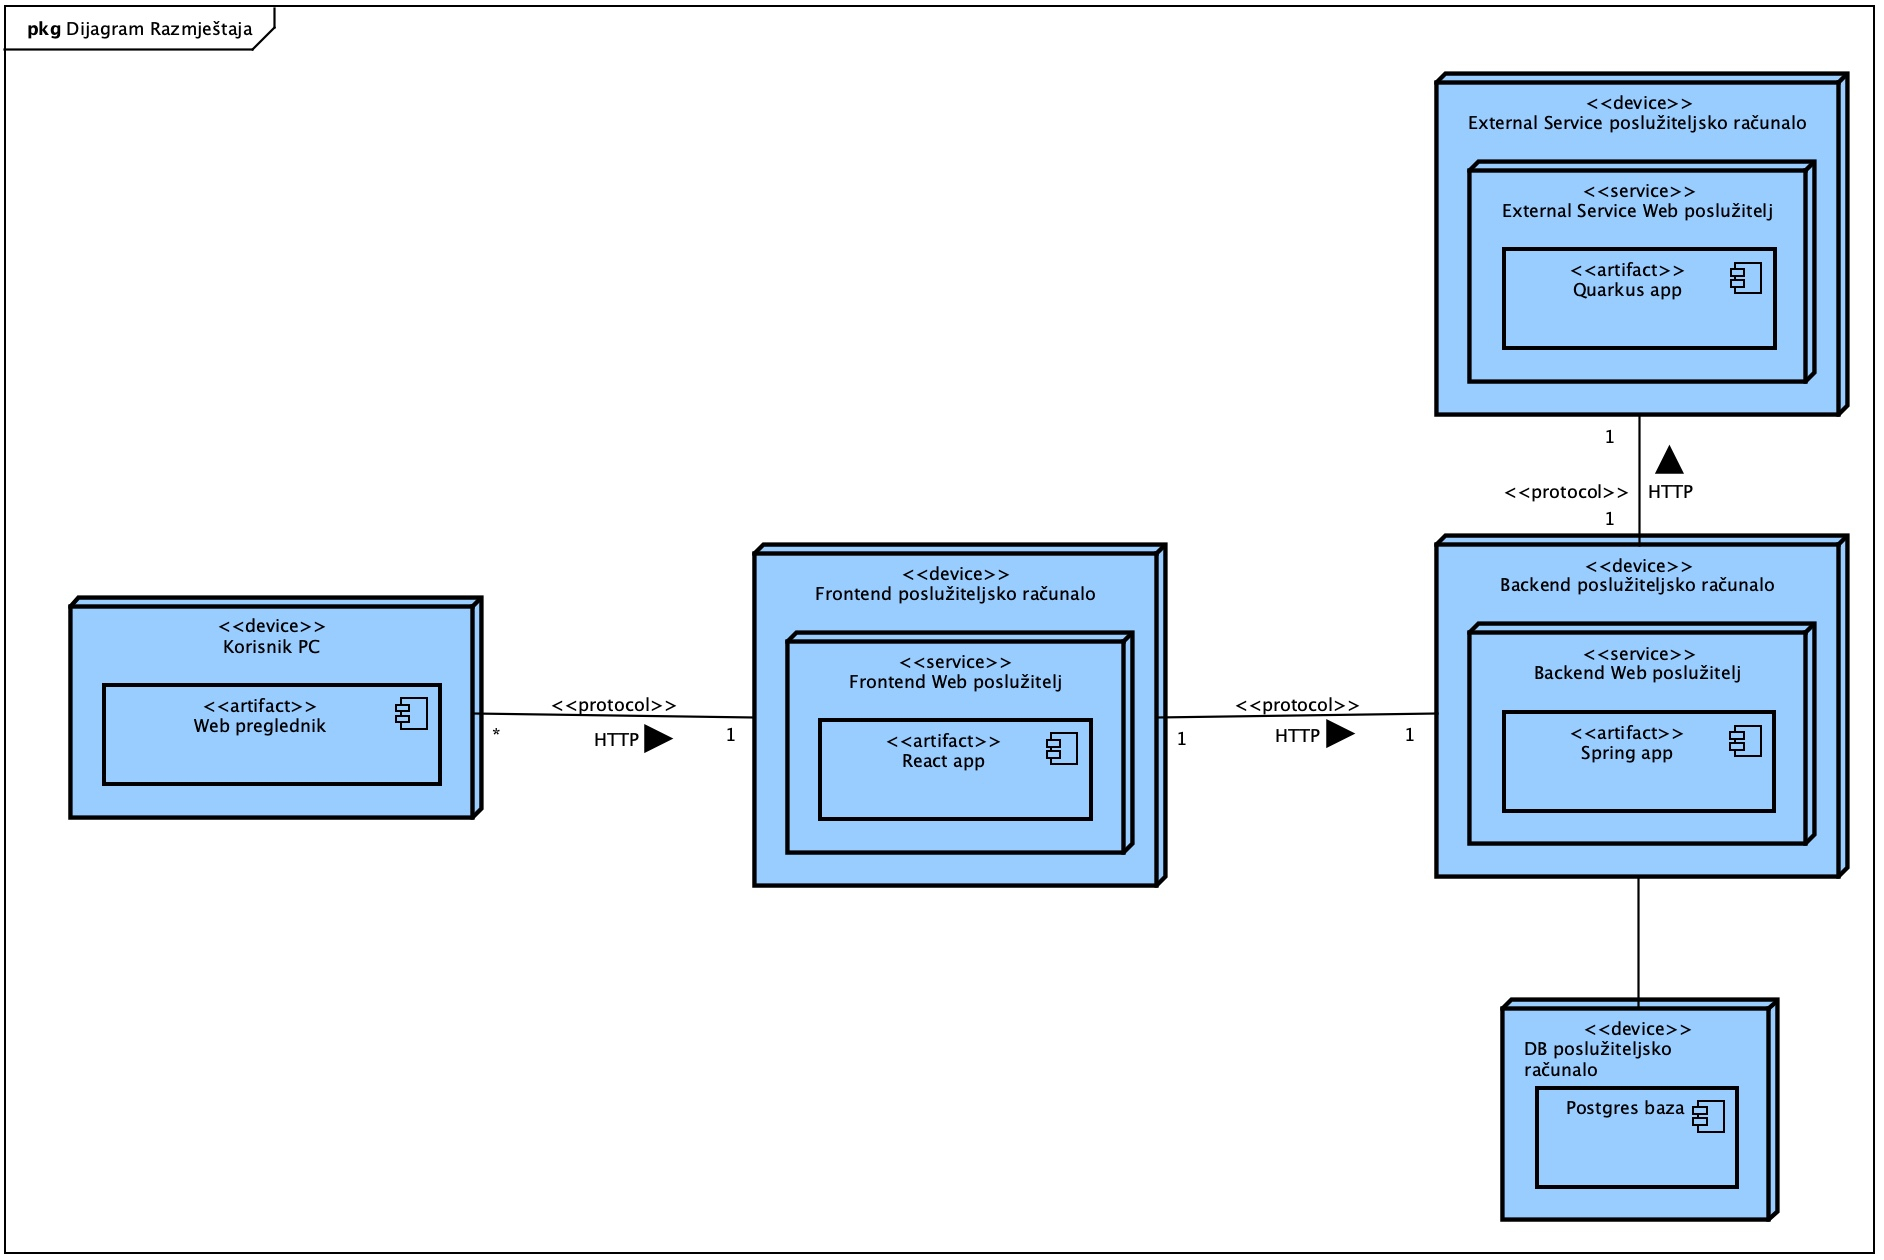
\includegraphics[scale=0.23]{slike/implementacija_dijagram_razmjestaja.jpg} %veličina slike u odnosu na originalnu datoteku i pozicija slike
				\centering
				\caption{Dijagram razmještaja}
				\label{fig:implementacija_dijagram_razmjestaja}
			\end{figure}
			
			\eject 
		
		\section{Upute za puštanje u pogon}
		
		Unutar korisničkog sučelja Render web aplikacije, nakon registracije, slijedite ove korake:
		
		\begin{enumerate}
			\item Kliknite na \textbf{``New''} i zatim \textbf{``Web service''} za kreiranje nove backend aplikacije, odnosno \textbf{``PostgreSQL''} za kreiranje nove aplikacije za bazu podataka.
			
			\item Odaberite opciju za povezivanje s repozitorijem na GitHubu. Preporučljivo je koristiti GitHub zbog integracije koju Render nudi. 
			
			\item Nakon povezivanja s GitHub računom, odaberite repozitorij u kojem se nalazi vaš projekt.
			
			\item Unutar sljedećeg prozora, potrebno je:
			\begin{itemize}
				\item Odrediti ime aplikacije.
				\item Odabrati regiju servera na kojoj će aplikacija biti upogonjena.
				\item Odrediti granu GitHub repozitorija.
				\item Napisati putanju do izvorne mape.
				\item Navesti putanju do \texttt{.dockerfile} datoteke potrebne Renderu za uspješno upogonjenje.
			\end{itemize}
			
			\item Odredite varijable okoline (\textit{environment variables}), koje su za ovaj projekt u sljedećem obliku:
			\begin{verbatim}
				spring.datasource.url=${DB_URL}
				spring.datasource.username=${DB_USERNAME}
				spring.datasource.password=${DB_PASSWORD}
			\end{verbatim}
			
			\item Nakon što je sve konfigurirano, pokrenite proces upogonjenja. Render će automatski preuzeti kod iz GitHub repozitorija, izgraditi aplikaciju prema definiranim komandama i pokrenuti aplikaciju.
			
			\item Za povezivanje s bazom podataka, Render nudi integraciju s različitim bazama podataka kao servisom. Možete kreirati novu instancu baze direktno preko Render sučelja i povezati je s vašom aplikacijom kroz varijable okoline.
			
			\item Nakon što je aplikacija pokrenuta, Render će pružiti URL na kojem je vaša aplikacija dostupna.
			
			\item Za promjene ili ažuriranje aplikacije, ažurirajte kod na GitHubu. Ukoliko ste tako odabrali u postavkama, Render će automatski detektirati promjene i ponovno upogoniti aplikaciju. Isti proces je moguć i ručno te u bilo kojem trenutku možete preusmjeriti render na neku drugu granu GitHub-a.
			
			\item Proces puštanja vanjskog servisa u pogon je identičan.
		\end{enumerate}
		
			
			\eject 
